\documentclass{wissdoc}
% Autor: Roland Bless 1996-2009, bless <at> kit.edu
% ----------------------------------------------------------------
% Diplomarbeit - Hauptdokument
% ----------------------------------------------------------------
%%
%% $Id: thesis.tex 65 2012-05-10 10:32:11Z bless $
%%
% wissdoc Optionen: draft, relaxed, pdf --> siehe wissdoc.cls
% ------------------------------------------------------------------
% Weitere packages: (Dokumentation dazu durch "latex <package>.dtx")
\usepackage[numbers,sort&compress]{natbib}
\usepackage{url}
%\usepackage{graphicx} 
% \usepackage{varioref}
% \usepackage{verbatim}
% \usepackage{float}    %z.B. \floatstyle{ruled}\restylefloat{figure}
% \usepackage{subfigure}
% \usepackage{fancybox} % für schattierte,ovale Boxen etc.
% \usepackage{tabularx} % automatische Spaltenbreite
% \usepackage{supertab} % mehrseitige Tabellen
% \usepackage[svnon,svnfoot]{svnver} % SVN Versionsinformation 
%% ---------------- end of usepackages -------------

%\svnversion{$Id: thesis.tex 65 2012-05-10 10:32:11Z bless $} % In case that you want to include version information in the footer

%% Informationen für die PDF-Datei
\hypersetup{
 pdfauthor={N.N.},
 pdftitle={Not set}
 pdfsubject={Not set},
 pdfkeywords={Not set}
}

% Macros, nicht unbedingt notwendig
%%%%%%%%%%%%%%%%%%%%%%%%%%%%%%%%%%%%%%%%%%%%%%%%%%%%%%%%%%
% macros.tex -- einige mehr oder weniger nuetzliche Makros
% Autor: Roland Bless 1998
%%%%%%%%%%%%%%%%%%%%%%%%%%%%%%%%%%%%%%%%%%%%%%%%%%%%%%%%%%
% $Id: macros.tex 33 2007-01-23 09:00:59Z bless $
%%%%%%%%%%%%%%%%%%%%%%%%%%%%%%%%%%%%%%%%%%%%%%%%%%%%%%%%%%


%%%%%%%%%%%%%%%%%%%%%%%
% Kommentare 
%%%%%%%%%%%%%%%%%%%%%%%
\ifnotdraftelse{
\newcommand{\Kommentar}[1]{}
}{\newcommand{\Kommentar}[1]{{\em #1}}}
% Alles innerhalb von \Hide{} oder \ignore{} 
% wird von LaTeX komplett ignoriert (wie ein Kommentar)
\newcommand{\Hide}[1]{}
\let\ignore\Hide

%%%%%%%%%%%%%%%%%%%%%%%%%
% Leere Seite ohne Seitennummer, wird aber gezaehlt
%%%%%%%%%%%%%%%%%%%%%%%%%

\newcommand{\leereseite}{% Leerseite ohne Seitennummer, n�chste Seite rechts (wenn 2-seitig)
 \clearpage{\pagestyle{empty}\cleardoublepage}
}
%%%%%%%%%%%%%%%%%%%%%%%%%%
% Flattersatz rechts und Silbentrennung, Leerraum nach rechts maximal 1cm
%%%%%%%%%%%%%%%%%%%%%%%%%%
\makeatletter
\newcommand{\myraggedright}{%
 \let\\\@centercr\@rightskip 0pt plus 1cm
 \rightskip\@rightskip
  \leftskip\z@skip
  \parindent\z@
  \spaceskip=.3333em
  \xspaceskip=.5em}
\makeatother

\makeatletter
\newcommand{\mynewline}{%
 \@centercr\@rightskip 0pt plus 1cm
}
\makeatother


%%%%%%%%%%%%%%%%%%%%%%%%%%
% F�r Index
%%%%%%%%%%%%%%%%%%%%%%%%%%
\makeatletter
\def\mydotfill{\leavevmode\xleaders\hb@xt@ .44em{\hss.\hss}\hfill\kern\z@}
\makeatother
\def\bold#1{{\bfseries #1}}
\newbox\dbox \setbox\dbox=\hbox to .4em{\hss.\hss} % dot box for leaders
\newskip\rrskipb \rrskipb=.5em plus3em % ragged right space before break
\newskip\rrskipa \rrskipa=-.17em plus -3em minus.11em % ditto, after
\newskip\rlskipa \rlskipa=0pt plus3em % ragged left space after break
\newskip\rlskipb \rlskipb=.33em plus-3em minus.11em % ragged left before break
\newskip\lskip \lskip=3.3\wd\dbox plus1fil minus.3\wd\dbox % for leaders
\newskip \lskipa \lskipa=-2.67em plus -3em minus.11em %after leaders
\mathchardef\rlpen=1000 \mathchardef\leadpen=600
\def\rrspace{\nobreak\hskip\rrskipb\penalty0\hskip\rrskipa}
\def\rlspace{\penalty\rlpen\hskip\rlskipb\vadjust{}\nobreak\hskip\rlskipa}
\let\indexbreak\rlspace
\def\raggedurl{\penalty10000 \hskip.5em plus15em \penalty0 \hskip-.17em plus-15em minus.11em}
\def\raggeditems{\nobreak\hskip\rrskipb \penalty\leadpen \hskip\rrskipa %
\vadjust{}\nobreak\leaders\copy\dbox\hskip\lskip %
\kern3em \penalty\leadpen \hskip\lskipa %
\vadjust{}\nobreak\hskip\rlskipa}
\renewcommand*\see[2]{\rlspace\emph{\seename}~#1} % from makeidx.sty

%%%%%%%%%%%%%%%%%%%%%%%%%%
% Neue Seite rechts, leere linke Seite ohne Headings
%%%%%%%%%%%%%%%%%%%%%%%%%%
\newcommand{\xcleardoublepage}
{{\pagestyle{empty}\cleardoublepage}}

%%%%%%%%%%%%%%%%%%%%%%%%%%
% Tabellenspaltentypen (benoetigt colortbl)
%%%%%%%%%%%%%%%%%%%%%%%%%%
\newcommand{\PBS}[1]{\let\temp=\\#1\let\\=\temp}
\newcolumntype{y}{>{\PBS{\raggedright\hspace{0pt}}}p{1.35cm}}
\newcolumntype{z}{>{\PBS{\raggedright\hspace{0pt}}}p{2.5cm}}
\newcolumntype{q}{>{\PBS{\raggedright\hspace{0pt}}}p{6.5cm}}
\newcolumntype{g}{>{\columncolor[gray]{0.8}}c} % Grau
\newcolumntype{G}{>{\columncolor[gray]{0.9}}c} % helleres Grau

%%%%%%%%%%%%%%%%%%%%%%%%%%
% Anf�hrungszeichen oben und unten
%%%%%%%%%%%%%%%%%%%%%%%%%%
\newcommand{\anf}[1]{"`{#1}"'}

%%%%%%%%%%%%%%%%%%%%%%%%%%
% Tiefstellen von Text
%%%%%%%%%%%%%%%%%%%%%%%%%%
% S\tl{0} setzt die 0 unter das S (ohne Mathemodus!)
% zum Hochstellen gibt es uebrigens \textsuperscript
\makeatletter
\DeclareRobustCommand*\textlowerscript[1]{%
  \@textlowerscript{\selectfont#1}}
\def\@textlowerscript#1{%
  {\m@th\ensuremath{_{\mbox{\fontsize\sf@size\z@#1}}}}}
\let\tl\textlowerscript
\let\ts\textsuperscript
\makeatother

%%%%%%%%%%%%%%%%%%%%%%%%%%
% Gau�-Klammern
%%%%%%%%%%%%%%%%%%%%%%%%%%
\newcommand{\ceil}[1]{\lceil{#1}\rceil}
\newcommand{\floor}[1]{\lfloor{#1}\rfloor}

%%%%%%%%%%%%%%%%%%%%%%%%%%
% Average Operator (analog zu min, max)
%%%%%%%%%%%%%%%%%%%%%%%%%%
\def\avg{\mathop{\mathgroup\symoperators avg}}

%%%%%%%%%%%%%%%%%%%%%%%%%%
% Wortabk�rzungen
%%%%%%%%%%%%%%%%%%%%%%%%%%
\def\zB{z.\,B.\ }
\def\dh{d.\,h.\ }
\def\ua{u.\,a.\ }
\def\su{s.\,u.\ }
\newcommand{\bzw}{bzw.\ }

%%%%%%%%%%%%%%%%%%%%%%%%%%%%%%%%%%%
% Einbinden von Graphiken
%%%%%%%%%%%%%%%%%%%%%%%%%%%%%%%%%%%
% global scaling factor
\def\gsf{0.9}
%% Graphik, 
%% 3 Argumente: Datei, Label, Unterschrift
\newcommand{\Abbildung}[3]{%
\begin{figure}[tbh] %
\centerline{\scalebox{\gsf}{\includegraphics*{#1}}} %
\caption{#3} %
\label{#2} %
\end{figure} %
}
\let\Abb\Abbildung
%% Abbps
%% Graphik, skaliert, Angabe der Position
%% 5 Argumente: Position, Breite (0 bis 1.0), Datei, Label, Unterschrift
\newcommand{\Abbildungps}[5]{%
\begin{figure}[#1]%
\begin{center}
\scalebox{\gsf}{\includegraphics*[width=#2\textwidth]{#3}}%
\caption{#5}%
\label{#4}%
\end{center}
\end{figure}%
}
\let\Abbps\Abbildungps
%% Graphik, Angabe der Position, frei w�hlbares Argument f�r includegraphics
%% 5 Argumente: Position, Optionen, Datei, Label, Unterschrift
\newcommand{\Abbildungpf}[5]{%
\begin{figure}[#1]%
\begin{center}
\scalebox{\gsf}{\includegraphics*[#2]{#3}}%
\caption{#5}%
\label{#4}%
\end{center}
\end{figure}%
}
\let\Abbpf\Abbildungpf

%%
% Anmerkung: \resizebox{x}{y}{box} skaliert die box auf Breite x und H�he y,
%            ist x oder y ein !, dann wird das uspr�ngliche 
%            Seitenverh�ltnis beibehalten.
%            \rescalebox funktioniert �hnlich, nur das dort ein Faktor
%            statt einer Dimension angegeben wird.
%%
% \Abbps{Position}{Breite in Bruchteilen der Textbreite}{Dateiname}{Label}{Bildunterschrift}
%

\newcommand{\refAbb}[1]{%
s.~Abbildung \ref{#1}}

%%%%%%%%%%%%%%%%%%%%
%% end of macros.tex
%%%%%%%%%%%%%%%%%%%%

% Print URLs not in Typewriter Font
\def\UrlFont{\rm}

\newcommand{\blankpage}{% Leerseite ohne Seitennummer, nächste Seite rechts
 \clearpage{\pagestyle{empty}\cleardoublepage}
}

%% Einstellungen für das gesamte Dokument

% Trennhilfen
% Wichtig! 
% Im ngerman-paket sind zusätzlich folgende Trennhinweise enthalten:
% "- = zusätzliche Trennstelle
% "| = Vermeidung von Ligaturen und mögliche Trennung (bsp: Schaf"|fell)
% "~ = Bindestrich an dem keine Trennung erlaubt ist (bsp: bergauf und "~ab)
% "= = Bindestrich bei dem Worte vor und dahinter getrennt werden dürfen
% "" = Trennstelle ohne Erzeugung eines Trennstrichs (bsp: und/""oder)

% Trennhinweise fuer Woerter hier beschreiben
\hyphenation{
% Pro-to-koll-in-stan-zen
% Ma-na-ge-ment  Netz-werk-ele-men-ten
% Netz-werk Netz-werk-re-ser-vie-rung
% Netz-werk-adap-ter Fein-ju-stier-ung
% Da-ten-strom-spe-zi-fi-ka-tion Pa-ket-rumpf
% Kon-troll-in-stanz
}

% Index-Datei öffnen
\ifnotdraft{\makeindex}
%%%%%%%%%%%%%% includeonly %%%%%%%%%%%%%%%%%%%
% Es werden nur die Teile eingebunden, die hier 
% aufgefuehrt sind!
\includeonly{%
titelseite,
erklaerung,
einleitung,
vorherige,
hardprog
}
%%%%%%%%%%%%%%%%%%%%%%%%%%%%%%%%%%%%%%%%%%%%%%
\begin{document}

\frontmatter
\pagenumbering{roman}
\ifnotdraft{
 %% Titelseite
%% Vorlage $Id: titelseite.tex 61 2012-05-03 13:58:03Z bless $

\def\usesf{}
\let\usesf\sffamily % diese Zeile auskommentieren für normalen TeX Font

\newsavebox{\Erstgutachter}
\savebox{\Erstgutachter}{\usesf Prof.~Dr.~H.~Schmeck}
\newsavebox{\Zweitgutachter}
\savebox{\Zweitgutachter}{\usesf Prof.~Dr.~?.~?????????}

\begin{titlepage}
\setlength{\unitlength}{1pt}
\begin{picture}(0,0)(85,770)

\includegraphics[width=\paperwidth]{logos/KIT_Deckblatt}
\end{picture}

\thispagestyle{empty}

%\begin{titlepage}
%%\let\footnotesize\small \let\footnoterule\relax
\begin{center}
\hbox{}
\vfill
{\usesf
{\huge\bfseries Energieoptimierung WLAN-basierter Ortungseinheiten \par}
\vskip 1.8cm
Masterarbeit\\
von\\[2mm]
\vskip 1cm

{\large\bfseries Marius Wodtke\\}
\vskip 1.2cm
Institut für Angewandte Informatik und Formale Beschreibungsverfahren (AIFB)\\
der Fakultät für Informatik\\
%Universität Karlsruhe (TH)\\[2ex]
\vskip 3cm
\begin{tabular}{p{5.5cm}l}
Erstgutachter: & \usebox{\Erstgutachter} \\
Zweitgutachter: & \usebox{\Zweitgutachter} \\
Betreuender~Mitarbeiter: & Dipl.-Inform.~K.~Bao \\
\end{tabular}
\vskip 3cm
Bearbeitungszeit:\qquad 01.~April~2017 -- 31.~Oktober~2017
}
\end{center}
\vfill
\end{titlepage}
%% Titelseite Ende


%%% Local Variables: 
%%% mode: latex
%%% TeX-master: "thesis"
%%% End: 

 \blankpage % Leerseite auf Titelrückseite
 %
 % Die folgende Erklärung ist für Diplomarbeiten Pflicht
 % (siehe Prüfungsordnung), für Studienarbeiten nicht notwendig
 \thispagestyle{empty}
\vspace*{32\baselineskip}
\hbox to \textwidth{\hrulefill}
\par
Ich erkl�re hiermit, dass ich die vorliegende Arbeit selbst�ndig verfasst und
keine anderen als die angegebenen Quellen und Hilfsmittel benutzt, 
die w�rtlich oder inhaltlich �bernommenen Stellen als solche kenntlich 
gemacht und die Satzung des KIT zur Sicherung guter wissenschaftlicher 
Praxis in der jeweils g�ltigen Fassung beachtet habe.

\vspace*{2cm}
Karlsruhe, den ??. ?????? 201?\hfill \hbox to 8cm{\hrulefill}

%%%%%%%%%%%%%%%%%%%%%%%%%%%%%%%%%%%%%%%%%%%%%%%%%%%%%%%%%%%%%%%%%%%%%%%%
%% Hinweis:
%%
%% Diese Erkl�rung wird von der Pr�fungsordnung f�r Diplom-, Master,
%% und Bachelorarbeiten verlangt und ist zu unterschreiben. 
%% F�r Studienarbeiten ist diese Erkl�rung nicht zwingend notwendig, 
%% schadet aber auch nicht.
%%%%%%%%%%%%%%%%%%%%%%%%%%%%%%%%%%%%%%%%%%%%%%%%%%%%%%%%%%%%%%%%%%%%%%%%
\clearpage







 \blankpage % Leerseite auf Erklärungsrückseite
}
%
%% *************** Hier geht's ab ****************
%% ++++++++++++++++++++++++++++++++++++++++++
%% Verzeichnisse
%% ++++++++++++++++++++++++++++++++++++++++++
\ifnotdraft{
{\parskip 0pt\tableofcontents} % toc bitte einzeilig
\blankpage
%\listoffigures
%\blankpage
%\listoftables
%\blankpage
}


%% ++++++++++++++++++++++++++++++++++++++++++
%% Hauptteil
%% ++++++++++++++++++++++++++++++++++++++++++
\graphicspath{{Bilder/}}

\mainmatter
\pagenumbering{arabic}
\chapter{Einleitung}
\label{ch:Einleitung}
Während die Ortung im Außenbereich fest in der Hand von Satellitennavigationssystemen wie dem Global Positioning System (GPS) liegen, existiert für die Ortung im Innenraum eine Vielzahl verschiedener Technologien. Neben Technologien wie Bluetooth, Radio Frequency Identification (RFID) und Ultra Wide Band (UWB) weckt WLAN wegen seiner großen Verbreitung immer wieder Interesse in Forschung und Industrie. 

So hat die Ortung mittels WLAN gerade im medizinischen Bereich durch kommerzielle Lösungen Verbreitung gefunden, Probleme finden sich aber bei Ortungsgenauigkeit gegenüber anderen Techniken und dem vergleichsweise hohen Energieverbrauch des WLAN-Protokolls.
Während sich viele wissenschaftliche Arbeiten der Ortungsgenauigkeit widmen, ist für den alltäglichen Einsatz die kurze Batterielaufzeit der mobilen Einheiten hinderlich, wenn nicht zum Beispiel Smartphones als mobile Einheiten in Frage kommen. 

Auch im Tunnelbau ist eine Ortung von Mitarbeitern und Besuchern von Nöten um in Notfällen bestimmen zu können, ob und wie viele Personen sich im Gefahrenbereich befinden. 
Dies beeinflusst die Arbeit der Rettungskräfte. 
Das veränderliche Umfeld der Baustelle, auf der große Stahl- und Betonelemente bewegt werden, stellt dabei die genaue Ortung mittels Radiowellen vor große Probleme und es wird nur eine Bereichsortung durchgeführt, bei der jede Tunnelröhre in mehrere hundert Meter große Abschnitte aufgeteilt wird und der Wechsel der Mitarbeiter zwischen den Abschnitten beobachtet wird. 
Dies stellt zwar nur eine geringe Genauigkeit dar, erlaubt es aber bei Bränden zu erkennen, welche Personen sich durch die Abschnitte Richtung Ausgang bewegen und welche in ihrem Abschnitt verharren. 
Solche Personen sind vermutlich bewegungsunfähig oder eingeschlossen.


\section{Bisherige Situation}
Die Ortung wird derzeit bei der Ed. Züblin AG mittels Bluetooth durchgeführt. 
Dabei sind die Basisstationen eigenständige Bluetooth-Einheiten, die mit dem Ethernet Backbone verbunden sind.
Als mobile Einheiten kommen sowohl batteriebetriebene "`Tags"' als auch Smartphones zum Einsatz. 
Das zentrale Sicherheitssystem fragt die gesehenen mobilen Einheiten bei den Basisstationen an und bereitet die Ergebnisse graphisch auf.

Der Tunnel wird in Bereiche zu circa 500 Meter aufgeteilt, die Tunnelbohrmaschine (TBM) stellt dabei einen Sonderbereich dar, weil sie sich im Gegensatz zu den anderen Bereichen langsam bewegt. 
Neue Bereiche werden hinter der TBM eingefügt und sind dann stationär.

Die Bluetooth-Basisstationen werden in Kästen verstaut, die weitere notwendige Technik, wie etwa ein Notfalltelefon, enthalten.
Weil diese Kästen nur etwa alle 500 Meter montiert sind, existieren große Lücken in denen die mobilen Einheiten nicht geortet werden.
Eine mobile Einheit wird im System so lange im selben Bereich angezeigt, bis sie wieder von einer Basisstation erkannt wird.

Wird die mobile Einheit von der Erfassungseinheit vor dem Portal (Tunneleingang) erkannt gilt sie als außerhalb des Tunnels.
Abbildung \ref{fig:bisherige} zeigt die bisherige Situation mit Bluetooth-Basisstaionen. 
Die Reichweite der der Basistationen ist dabei nicht maßstabsgetreu.

\begin{figure}[h]
  \centering
	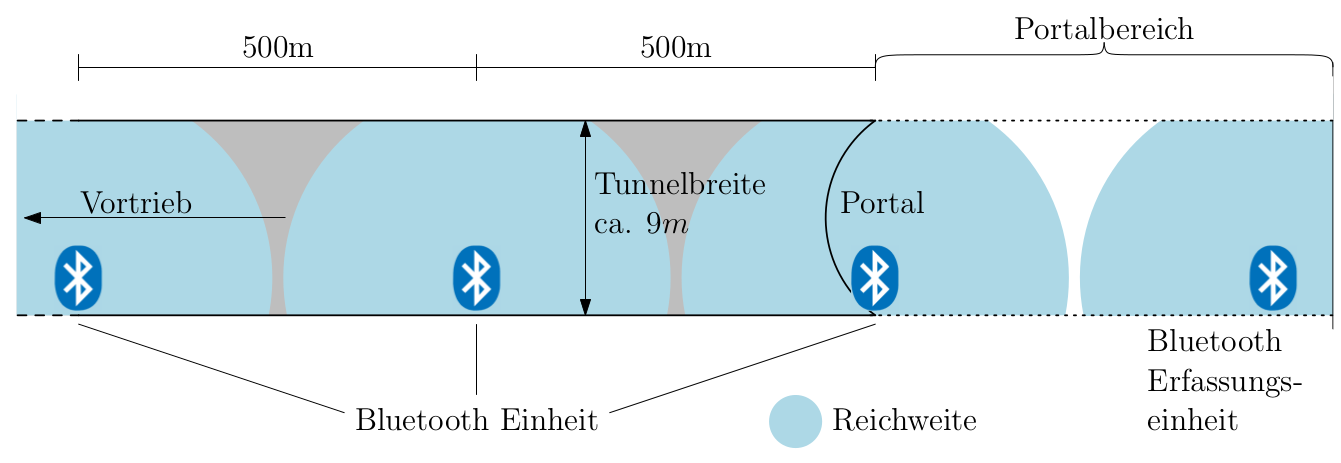
\includegraphics[width=\textwidth]{images/bisherige.png}
  \caption{Bereichsortung mit Bluetooth, aus \cite{maurer2016unterstuetzung}.}
  \label{fig:bisherige}
\end{figure}

 
\section{Umgebung für funkbasierte Ortung}
Als Versuchsumgebung dient die Tunnelbaustelle Rastatt.
Dort gelten die Positionen der Kästen für die Technik als unveränderlich.
Nur sie bieten Strom, Netzwerkanbindung (LAN) und Schutz vor dem Baustellenumfeld.
Für Funkprotokolle, die weniger als 250 Meter Reichweite entfalten muss daher mit Erfasssungslücken gerechnet werden.
Auf der TBM und anderen technischen Fahrzeugen sind jedoch mehr Basisstationen möglich.

Es existiert bereits ein WLAN-Netzwerk, dessen Access Points als Basisstationen genutzt werden können.
Es handelt sich um APs der Firma Lancom, diese stellt auch ein Modell LN-862 für Versuche.
Für zukünftige Baustellen soll der Abstand der Versorgungskästen auf 250 Meter sinken. 
Diese Situation ist in Abbildung \ref{fig:zukuenftige} skizziert.

\begin{figure}[h]
  \centering
	\includegraphics[width=\textwidth]{images/zukuenftige.eps}
  \caption{Zukünftige Situation der Tunnelbaustellen.}
  \label{fig:zukuenftige}
\end{figure}

\section{Problemstellung}
Es muss ein System geschaffen werden, welches Mitarbeiter einem 250 Meter langen Abschnitt innerhalb eines im Bau befindlichen Tunnels zuordnet.
Dazu soll keine Nutzerinteraktion nötig sein, der Nutzer wird wird über eine mobile Einheit geortet.
Die Ortung muss unterirdisch funktionieren und robust gegenüber Stahlhindernissen sein.
Außerdem können Basisstation für die Ortung nur alle 250 Meter platziert werden.


\section{Zielsetzung der Arbeit}
\label{ch:Einleitung:sec:Zielsetzung}
Ziel der Arbeit soll der Entwurf und die Implementierung eines Bereichsortungssystems für Personen in Tunnelanlagen sein. 
Bei einem Bereichsortungssystem handelt es sich um ein Ortungssystem, bei dem die Positionen nicht genau bestimmt werden. 
Stattdessen wird das Areal, auf dem geortet werden soll, in einzelne Bereiche unterteilt und jede mobile Einheit beim Vorgang des Ortens einem dieser Bereiche zugeordnet.

Diese Arbeit grenzt sich von vorherigen Arbeiten dadurch ab, dass die Laufzeit beziehungsweise der Energieverbrauch der mobilen Einheiten im Vordergrund steht. 
Ziel dieser Arbeit ist eine mehrmonatige Laufzeit der mobilen Einheiten. 

Für diese Arbeit werden mehrere Prototypen für mobile Einheiten entwickelt und auf ihre Charakteristik bezüglich des Energieverbrauchs und der Erkennungszuverlässigkeit untersucht.
Der Entwurfsraum umfasst dabei die Hardware und Software der mobilen Enheit sowie die Implementierung des Ortungsdienstes. 
Die für die Funktechnologie benötigte Infrastruktur wird jeweils als gegeben angenommen.


\section{Anforderungen an das Bereichsortungssystem}
\label{ch:Einleitung:sec:Anforderungen}
Da es sich um ein Bereichsortungssystem handeln soll, werden keine direkten Anforderungen an die Genauigkeit der Ortung gestellt. 
Jedoch soll ein klarer Wechsel zwischen zwei Bereichen, und damit zwei Basisstationen, zuverlässig erkannt werden. 
Die mobilen Einheiten sollen von Personen um den Hals getragen werden können. 
Dies bedingt ein geringes Gewicht des Akkus, gleichzeitig soll aber die Laufzeit der mobilen Einheit maximiert werden, sodass ein Akku mit möglichst großer Kapazität gewählt werden sollte.
Zuletzt soll unter Rücksichtnahme auf das beschriebene Szenario die Komplexität der benötigten IT-Infrastruktur so gering wie möglich gehalten werden um ein stabiles und kostengünstiges System zu garantieren. 


\section{Gliederung der Arbeit}
\label{ch:Einleitung:sec:Gliederung}
Nachdem zunächst in Kapitel \ref{ch:Grundlagen} die Grundlagen der funkbasierten Ortung und der verwendeten Funkprotokolle behandelt werden, wird in Kapitel \ref{ch:Analyse} das Problem analysiert und verwandte Arbeiten aufgezeigt.
Kapitel \ref{ch:Implementierung} beschäftigt sich mit der Implementierung und Untersuchung der Prototypen. 
Das Fazit in Kapitel \ref{ch:Fazit} fasst die Arbeit noch einmal zusammen, vergleicht und bewertet die Ergebnisse.
  % Einleitung
%TODO Bluetooth Beispiel

\chapter{Vorherige Arbeiten}
\label{ch:Vorherige}
%% ==============================
In diesem Kapitel werden vorhandene Lösungen, die für die gegebene Aufgabe der Bereichsortung in Tunneln in Frage kommen, diskutiert. 
Es werden hauptsächlich Lösungen auf Basis der 802.11 Spezifikation ausgewählt, dabei aber auch solche Systeme einbezogen, die eine spezifische Position der mobilen Einheit angeben, da diese anschließend trivial einem Bereich zugeordnet werden kann. 
Es werden sowohl wissenschaftliche als auch kommerzielle Lösungen diskutiert.\\
Auffällig ist bei der Recherche, dass wissenschaftliche Veröffentlichungen sich fast immer auf eines von zwei Aufgabenfeldern beziehen: Entweder soll die Ortungsgenauigkeit erhöht oder die Anforderungen ohne signifikanten Genauigkeitsverlust gesenkt werden. 
Diese Anforderungen können zum Beispiel Komplexität des Knoten-Netzwerks, des einzelnen Knotens, Synchronisation oder vorherige Kalibrierung sein.\\
An den Energieverbrauch der mobilen Einheiten werden üblicherweise keine Forderungen gestellt und oft von den Veröffentlichungen komplett ignoriert.
Dies ist akzeptabel wenn davon ausgegangen wird, dass die mobile Einheit zusätzlichen Nutzen bietet und das Laden der Einheit in Nutzungsszenario des Anwenders bereits vorgesehen ist.
So hat der Anwender in einem Szenario, bei dem sein Smartphone mittels direkter oder indirekter Selbstlokalisierung seine Position bestimmt um ihn zu navigieren nur minimale Anforderungen an den Energieverbrauch.
In Szenarien mit direkter oder indirekter Fernlokalisierung hat die mobile Einheit für den Anwender oft keinen direkten Nutzen, deshalb ist eine Forderung nach täglichem oder wöchentlichem Laden beziehungsweise Wechseln der Batterie schwerer durchzusetzen.\\





\subsection{Ultraschall}
Skibiniewski et al. nutzen Ultraschall für eine Fernlokalisierung mit TOF \cite{skibniewski2009simulation}.
Ultraschall kann nicht von WLAN APs empfangen werden und es muss zusätzliche Hardware installiert werden, das System soll hier dennoch Beachtung finden, da es für die Ortung von Baumaterial auf Baustellen entwickelt wurde.\\
Bei diesem System sendet zunächst der Knoten einen Beacon Frame der ZigBee Spezifikation (802.15.4) an die mobile Einheit, diese antwortet und sendet unmittelbar danach das Ultraschallsignal.
Das schnelle 2.4GHz ZigBee Signal dient dem Knoten dann als Referenz für den Sendezeitpunkt des Ultraschallsignals, welches wegen seiner langsamen Ausbreitungsgeschwindigkeit $c \approx 343m/s$ wesentlich weniger anfällig für ungenaue Zeitstempel ist. 
Außerdem kann die Zeit zwischen dem Aussenden des Beacon Frames und der Antwort gemessen werden um zusätzliche TOF-Informationen zu gewinnen. \\
Statt ZigBee ließe sich auch WLAN nutzen, ZigBee ist jedoch bereits auf niedrigen Energieverbrauch ausgelegt und wegen des Ultraschalls wäre trotzdem ein extra Knoten nötig.
Problematisch an der Lösung ist entweder der Energieverbrauch der Ultraschalleinheit oder die Reichweite, ausreichend kleine Einheiten reichen keine 100m weit und leiden trotzdem unter kurzer Batterielaufzeit.
Die Autoren schließen deshalb, dass noch Innovation in diesem Bereich notwendig ist um dieses System praktikabel zu machen.

\section{LANDMARC}
\label{ch:Vorherige:sec:LANDMARC}
Ni et al. stellen ein Ortungssystem auf Basis von Radio Frequency Identification (RFID) vor \cite{ni2004landmarc}.
Dazu werden aktive RFID-Tags als mobile Einheiten eingesetzt, diese sind mit einer Batterie ausgestattet und senden regelmäßig ihre gespeicherte ID aus.\\
Der Knoten ist mit einem Lesegerät (RFID-Reader) ausgestattet und empfängt die ID, der Knoten liefert dann die ID und ein Signalstärkelevel zwischen 1 und 8 zurück. 
Da das Signalstärkelevel nur eine sehr grobe Auflösung hat verbessern Ni et al. die Genauigkeit durch das Ausbringen von zusätzlichen Tags an bekannten, fixen Positionen, für die Bereichsortung ist dies aber nicht notwendig.\\
Die Autoren geben für ein Sendeintervall von 7,5 Sekunden eine Batterielaufzeit von 3-5 Jahren an, dabei sind die Tags klein genug und könnten, wie in der Einleitung gefordert, an einem Band um den Hals getragen werden.
%"System lässt sich leicht auf Bluetooth übertragen"

\section{Bluetooth}
\label{ch:Vorherige:sec:Bluetooth}
Hier habe ich noch kein Paper, es kommt aber fix noch mindestens ein System auf Bluetooth-Basis + Kritik an verschiedenen Buetooth Parametern.



\chapter{Hardware \& Programmiermöglichkeiten}
\label{ch:hardprog}
In diesem Kapitel soll die für die mobilenen Einheiten verwendete Hardware und ihre Programmiermöglichkeiten näher beleuchtet werden.
Als mobile Einheiten werden in dieser Arbeit hauptsächlich Tags behandelt: Tags sind kleine Geräte, die ausschließlich zur Ortung und demit einhergehender Identifikation genutzt werden.\\
Diese Arbeit behandelt jedoch ebenfalls die Ortung mittels Smartphones mit dem Android Betriebssystem von Google \cite{google2017android}, um diese in das System einzugliedern und bei Personen, die ein Firmenhandy besitzen die Notwendigkeit eines zusätzlichen Tags zu eliminieren.
Dabei sollte der Energieverbrauch nicht zu hoch sein, es werden jedoch nicht die selben Beschränkungen bezüglich der Batterielaufzeit, da es in der natürlichen Erwartung des Nutzers liegt, dass ein Smartphone häufiger geladen werden muss.
Allerdings muss ein Smartphone mindestens eine 12-stündige Schicht ohne Ladevorgang auskommen, da sonst ein Bereichswechsel nicht mehr festgestellt werden könnte.

\begin{figure}[h]
  \centering
	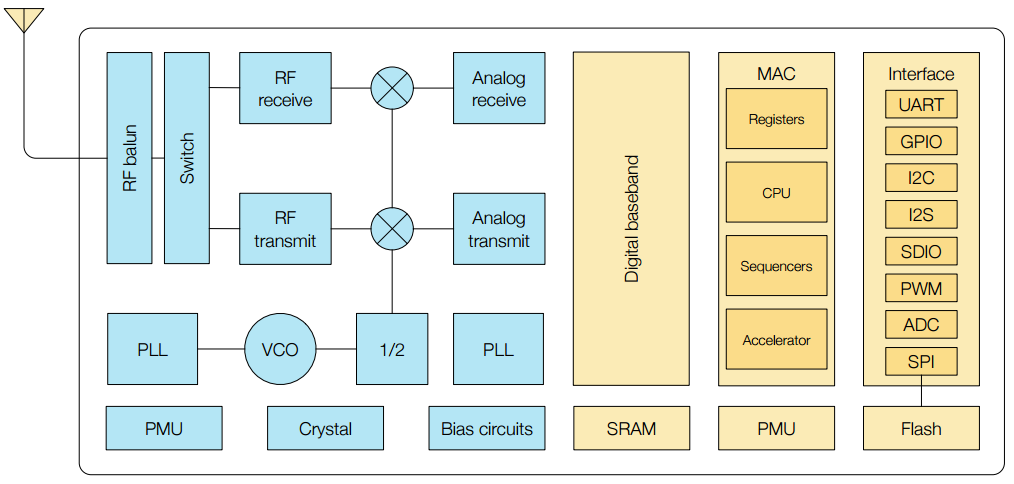
\includegraphics[width=\textwidth]{images/espblock.png}
  \caption{Blockdiagramm des ESP8266, aus \cite{espressif2017esp8266}}
  \label{fig:espblock}
\end{figure}

\section{ESP8266}
Für WLAN-basierte Tags kommt der ESP8266 von Espressif in den Modulen ESP12-S beziehungsweise ESP12-F zum Einsatz.
Der ESP8266 zeichnet sich durch einen niedrigen Energieverbrauch und viele Freiheiten bei der Programmierung aus, die Module ESP12-S und ESP 12-F unterscheiden sich dabei hauptsächlich durch ihre Antenne, siehe Abb. \ref{fig:espmodules}.
Der neuere ESP12-F sollte eine höhere Reichweite entfalten, dies wird noch Gegenstand eines Experiments sein.\\
Der Esp8266 besitzt neben einer CPU eine 802.11b/g/n/e/i-fähige WLAN-Einheit und diverse andere, kabelgebundene Kommunikationsstandards wie zum Beispiel GPIO, I2C und SPI, siehe Abb. \ref{fig:espblock}.
Der Chip selbst besitzt weder einen Flashspeicher für Programme und Daten noch eine Antenne, diese werden auf dem Modul, z.B. ESP-12F, integriert \cite{espressif2017esp8266}.
Espressif gibt im Datenblatt auch Aufschluss über den Energieverbrauch des Chips, siehe dazu Abb. \ref{fig:esppower}.




\begin{figure}[h]
  \centering
	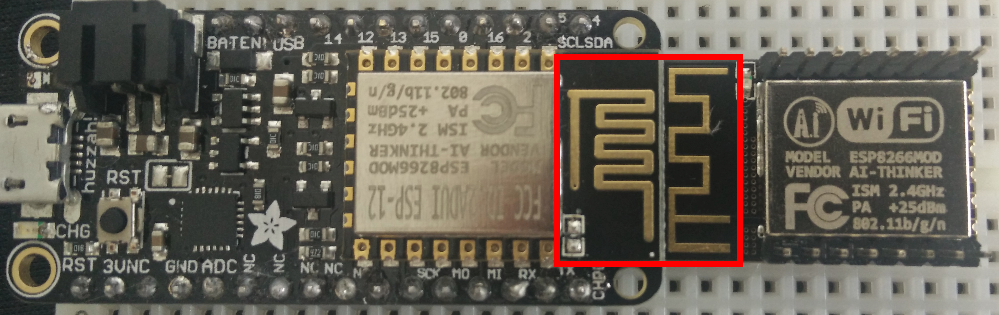
\includegraphics[width=\textwidth]{images/espmodules.png}
  \caption{Vergleich der Antennen, links: ESP12-S verbaut auf einem Adafruit Feather Huzzah, rechts: ESP12-F}
  \label{fig:espmodules}
\end{figure}

\begin{figure}[h]
  \centering
	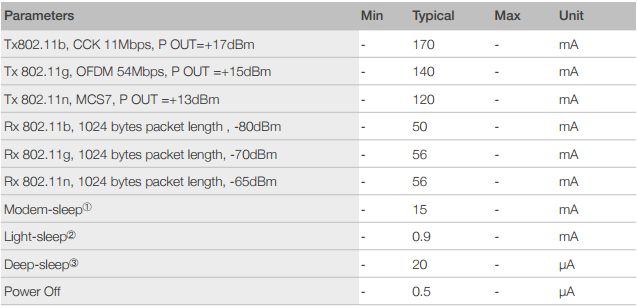
\includegraphics[width=\textwidth]{images/esppower.png}
  \caption{Energieverbrauch des ESP8266 bei verschiedenen Operationen, aus \cite{espressif2017esp8266}}
  \label{fig:esppower}
\end{figure}

\section{Texas Instruments SensorTag}
Für das Bluetooth-basierte Tag wird das SensorTag von Texas Instruments verwendet.



%% ++++++++++++++++++++++++++++++++++++++++++
%% Anhang
%% ++++++++++++++++++++++++++++++++++++++++++

\appendix
%\include{anhang_a}
%\include{anhang_b}

%% ++++++++++++++++++++++++++++++++++++++++++
%% Literatur
%% ++++++++++++++++++++++++++++++++++++++++++
%  mit dem Befehl \nocite werden auch nicht 
%  zitierte Referenzen abgedruckt
\cleardoublepage
\phantomsection
\addcontentsline{toc}{chapter}{\bibname}
%%
\nocite{*} % nur angeben, wenn auch nicht im Text zitierte Quellen 
           % erscheinen sollen
\bibliographystyle{itmabbrv} % mit abgekürzten Vornamen der Autoren
%\bibliographystyle{gerplain} % abbrvnat unsrtnat
% spezielle Zitierstile: Labels mit vier Buchstaben und Jahreszahl
%\bibliographystyle{itmalpha}  % ausgeschriebene Vornamen der Autoren
\bibliography{thesis}
%% ++++++++++++++++++++++++++++++++++++++++++
%% Index
%% ++++++++++++++++++++++++++++++++++++++++++
\ifnotdraft{
\cleardoublepage
\phantomsection
\printindex            % Index, Stichwortverzeichnis
}
\end{document}
%% end of file
